\section{Server Implementation}
 
\frame{\sectionpage}
 
\begin{frame}[fragile]{Initializing Spark DataFrame and Flask}
	\begin{verbatim}
	print("### Initializing Spark Context")
	sc, sql_ctx, spark = init_spark("Spark_Webserver", "local[4]")
	
	print("### Creating Spark dataframe from file")
	df = spark.read.json("quotes-table.json")
	
	print("### Initializing Flask app")
	app = Flask(__name__)
	\end{verbatim}
\end{frame}
	
\begin{frame}[fragile]{Using Spark to run dataframe query}
	\begin{verbatim}
	# Get author parameter from url (ex: [server-ip]/?author=tesla)
	author_arg = request.args.get('author', default = "", 
	    type = str).lower().strip()
	
	# Get all rows where author column string contains 
	# author_arg substring
	author_quotes = df.filter(
	    lower(df.author).like("%" + author_arg + "%"))
	\end{verbatim}
\end{frame}

\begin{frame}[fragile]{Using Flask to return the web request as JSON}
	\begin{verbatim}
	# Generate random number for row index
	random_row = random.randint(0, num_quotes - 1)
	
	# Collect table rows, converting that dataframe to a python list
	rows = author_quotes.collect()
	
	# Retrieve the random row's quote and author
	quote = str(rows[random_row]["quote"])
	author = str(rows[random_row]["author"])
	
	# Return response
	return '{"quote":"' + quote + '", "author":"' + author + '"}'
	\end{verbatim}
\end{frame}

\begin{frame}{Quotes database}
	\begin{figure}
		\centering
		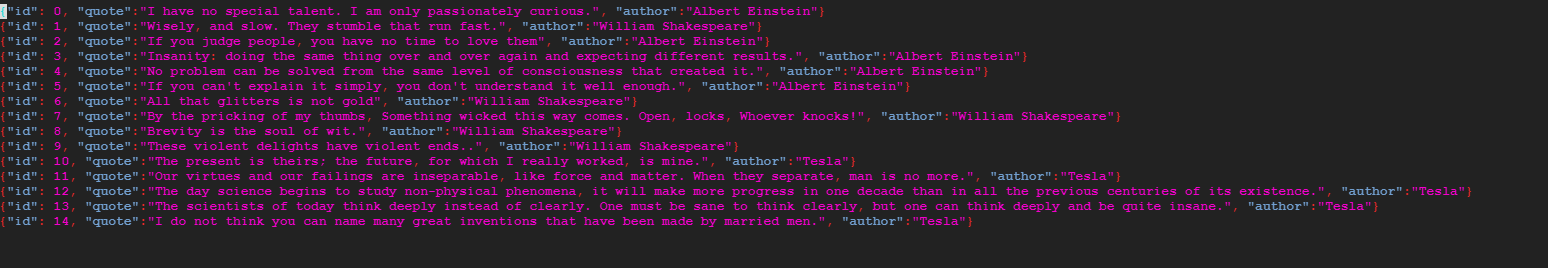
\includegraphics[width =1\linewidth]{robot-spark-proj/quotes-table.PNG}
		\caption{quotes-database.json file}
	\end{figure}
	
\end{frame}

